\begin{homeworkProblem}

Sampling from probability distributions. Show histograms and compare them to corresponding PDFs.

(a) Sampling from the standard Normal distribution with both the Box-Muller method and the Acceptance-Rejection method. Discuss the pros and cons of both methods. \\
(b) Sampling from the distribution with the following pdf:
$$f(x) \propto \exp \left(-\frac{1}{2} x^2\right)\left(\sin ^2(6 x)+3 \cos ^2(x) \sin ^2(4 x)+1\right)$$

\textcolor{blue}{Solution} \\

(a)
We could see that $X,Y\stackrel{i.i.d.}{\sim}\N(0,1)$, the estimated correlation coefficient is getting closer to, and the sampled distribution is getting closer to the theoretical distribution as the number of samples increases.\\

\begin{figure}[h]
    \centering
    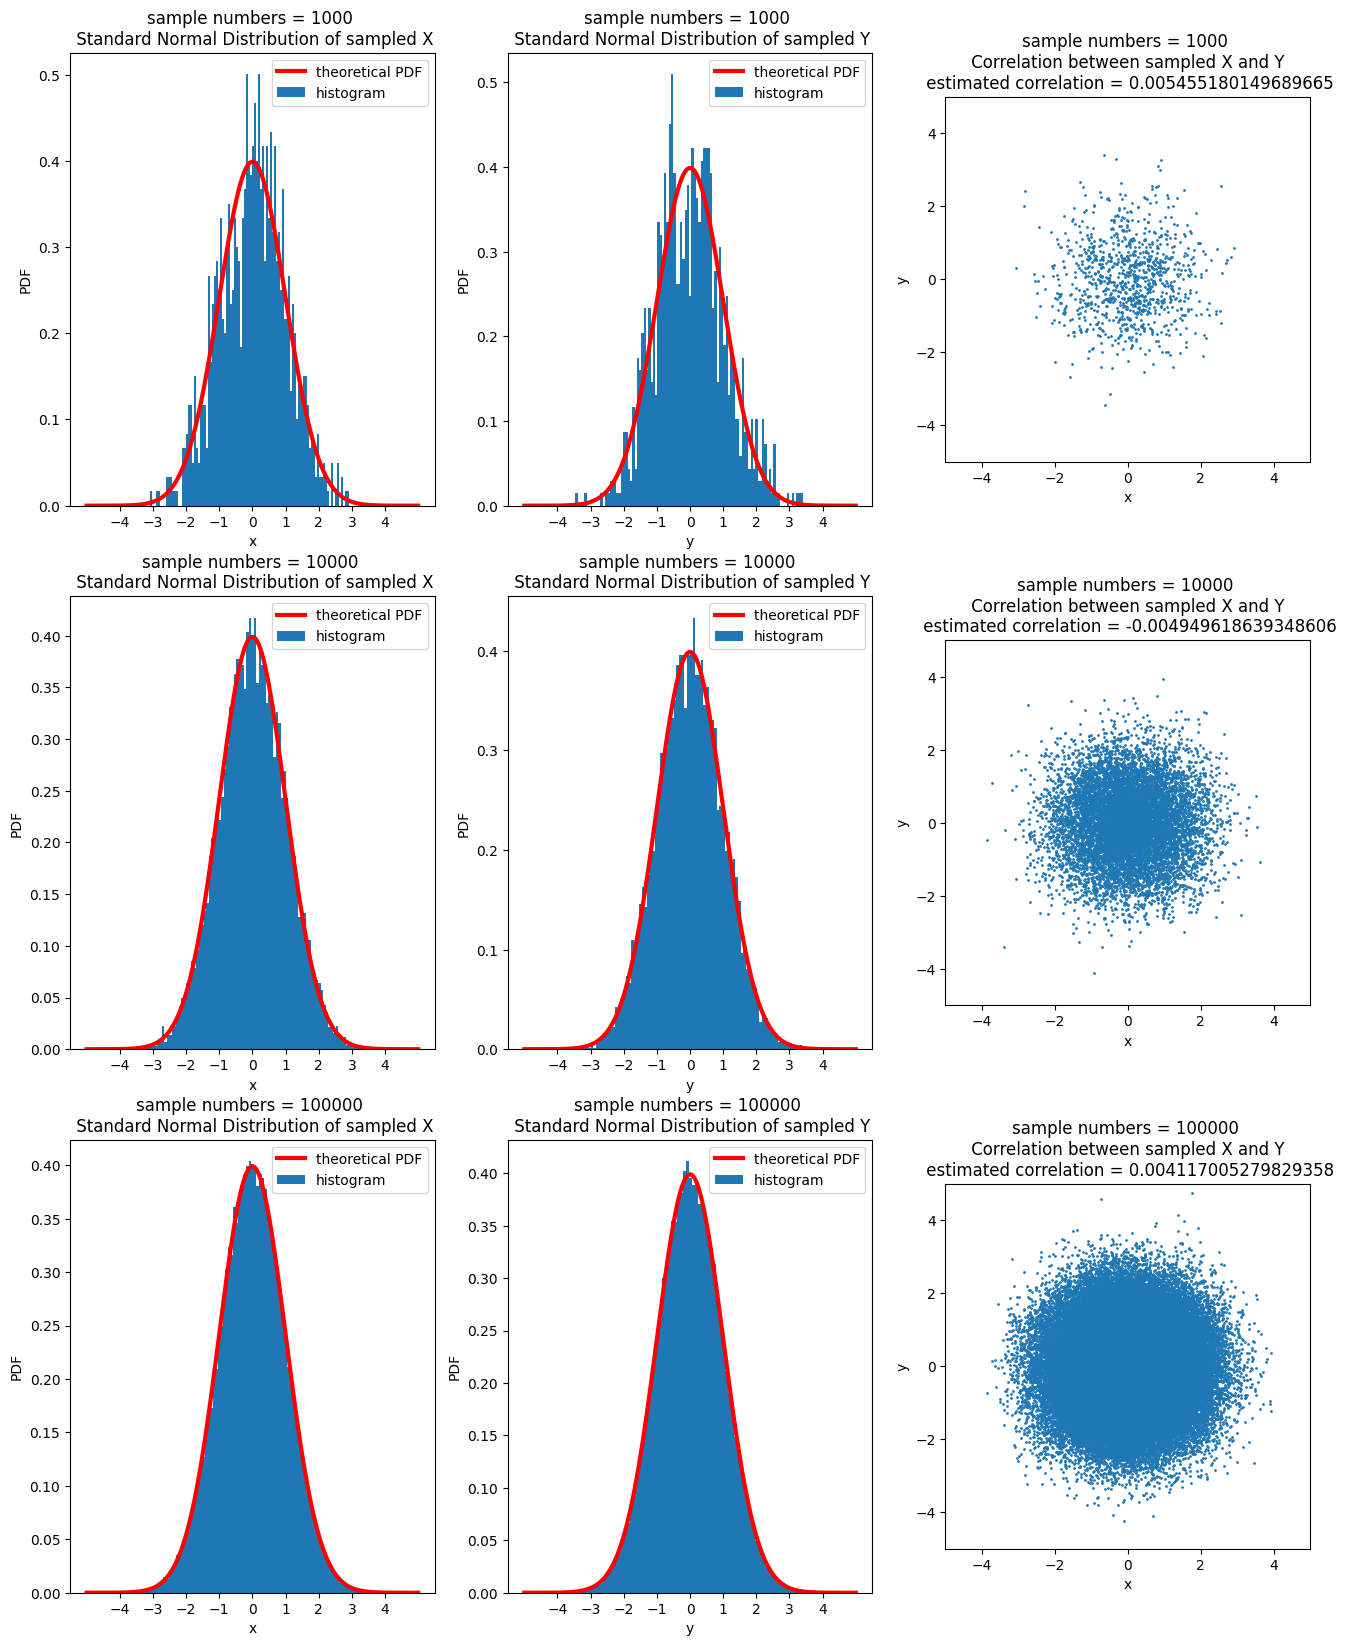
\includegraphics[height=0.55\textheight]{./figure/p5/box_muller.png}
    \caption{Sample $\N(0,1)$ with Box-Muller method}
\end{figure}


(b) Similarly with (a), we want to sample on $\N(0,1)$ with acceptance-rejection algorithm. \\
Let $Z\sim \N(0,1)$, and $X=|Z|$. \\
So $Z\in (-\infty,+\infty)$, $X\in (0,+\infty)$. \\
We can calculate the PDF of $X$: \\
$f(x)=f_X(x)=\dfrac{2}{\sqrt{2\pi}}e^{-\frac{1}{2}x^2},x>0$. \\

And we can choose that $Y\sim Expo(1)$, and its PDF is $g(y)=f_Y(y)=e^{-y},y>0$. \\
Following the method in (a), we can get that $c\geq sup_y\dfrac{f(y)}{g(y)}$. \\
$\dfrac{f(y)}{g(y)}=\dfrac{\frac{2}{\sqrt{2\pi}}e^{-\frac{1}{2}y^2}}{e^{-y}}=\dfrac{2}{\sqrt{2\pi}}e^{-\frac{1}{2}y^2+y}$. \\
Since $y>0$, so we can get that when $y=1$, $\dfrac{f(y)}{g(y)}$ will take the maximum value within the domain. \\
i.e. $sup_y\dfrac{f(y)}{g(y)}=\dfrac{f(1)}{g(1)}=\dfrac{2}{\sqrt{2\pi}}e^{-\frac{1}{2}+1}=\sqrt{\dfrac{2e}{\pi}}$. \\
So we can just take $c=\sqrt{\dfrac{2e}{\pi}}$. \\

Then we can do the acceptance-rejection algorithm. \\
1. Generate $Y\sim Expo(1)$. \\
2. Generate $U\sim Unif(0,1)$. \\
3. If $U\leq \dfrac{f(Y)}{c\cdot g(Y)}=\dfrac{\frac{2}{\sqrt{2\pi}}e^{-\frac{1}{2}Y^2}}{\sqrt{\frac{2e}{\pi}}\cdot e^{-Y}}=\dfrac{1}{\sqrt{e}}e^{-\frac{1}{2}Y^2+Y}=e^{-\frac{1}{2}(Y-1)^2}$, then set $X=Y$ \\
4. Else, go back to step 1. \\

After that, we can get the sample the distribution of $X$. \\
To sample on $Z\sim \N(0,1)$, since $X=|Z|$, so we can generate $U'\sim Unif(0,1)$, \\
and let $Z=\begin{cases}
    X, & U'\leq \frac{1}{2} \\
    -X, & U'>\frac{1}{2}
\end{cases}$. \\
After that, we can sample the distribution of $Z\sim \N(0,1)$ with acceptance-rejection method. \\

\begin{figure}[h]
    \centering
    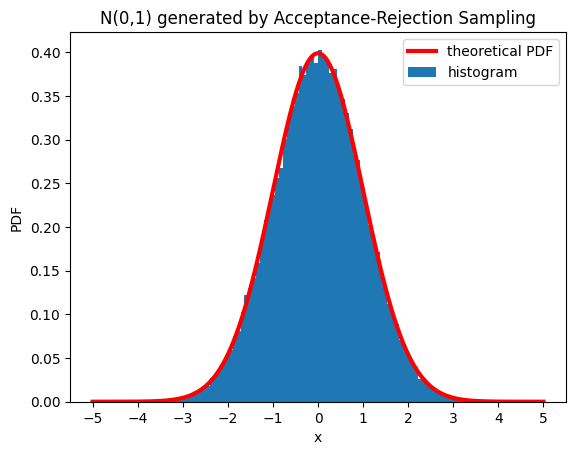
\includegraphics[width=0.5\textwidth]{./figure/p5/accept_reject.png}
    \caption{Sample $\N(0,1)$ with Acceptance-Rejection method}
\end{figure}

Prove the correctness of the algorithm in theorem:\\
1. Let event $A = "U \leq \dfrac{f(Y)}{c\cdot g(Y)}"$.\\
From the decription of the algorithm, we know that we let $X=Y$ when $A$ happens.\\
So the PDF of generated r.v.s. $X$ is that $f_Y(y|A)=\dfrac{P(A|Y=y)}{P(A)}\cdot f_Y(y)$.

2. And $P(A|Y=y)=P(U\leq \dfrac{f(Y)}{c\cdot g(Y)}|Y=y)=P(U\dfrac{f(y)}{c\cdot g(y)}|Y=y)$.\\
Since $U$ and $Y$ are independent, so $P(U\leq \dfrac{f(y)}{c\cdot g(y)}|Y=y)=P(U\leq \dfrac{f(y)}{c\cdot g(y)})$.\\
And since $U\sim Unif(0,1)$, so $P(U\leq \dfrac{f(y)}{c\cdot g(y)})=\dfrac{f(y)}{c\cdot g(y)}$.\\
So $P(A|Y=y)=\dfrac{f(y)}{c\cdot g(y)}$.

3. As for $P(A)$, with LOTP, we can get that\\
$P(A)=\int_{0}^{+\infty}P(A|Y=y)g(y)dy$.\\
From 2., we get that $P(A|Y=y)=\dfrac{f(y)}{c\cdot g(y)}$.\\
So $P(A)=\int_{0}^{+\infty}\dfrac{f(y)}{c\cdot g(y)}g(y)dy=\dfrac{1}{c}\int_{0}^{+\infty}f(y)dy=\dfrac{1}{c}$.\\
For the last step, this is because $g(y)$ is the PDF of $Expo(1)$, which support is $(0,+\infty)$, so $\int_{0}^{+\infty}g(y)dy=1$.

4. Combine 2., 3. into 1., we can get that\\
$P(Y=y|A)=\dfrac{P(A|Y=y)}{P(A)}\cdot f_Y(y)=\dfrac{\frac{f(y)}{c\cdot g(y)}}{\frac{1}{c}}\cdot g(y)=f(y)$.

So from 1. to 4., we have prove that the PDF of generated r.v.s. $X$ is that $f_Y(y|A)=f(y)$.\\
i.e. $X\sim f(y)$.

And since $X=|Z|$, so we generated a r.v.s. $U'\sim (0,1)$.\\
And let $Z=\begin{cases}
    X, & U'\leq \frac{1}{2}\\
    -X, & U'>\frac{1}{2}
\end{cases}$.

This is because $Z\sim(0,1)$, so it is symmetric about $x=0$.\\
And since $X=|Z|$, so it can be regard that $X$ takes the value of $Z$ with probability $\frac{1}{2}$, and takes the value of $-Z$ with probability $\frac{1}{2}$.\\
So we can generate $X$ with $U'\sim (0,1)$, and let $X=Z$ when $U'\leq \frac{1}{2}$, and let $X=-Z$ when $U'>\frac{1}{2}$.

So above all, we can generate $Z\sim \N(0,1)$ with acceptance-rejection method. The correctness have been proved.\\

(c) Both Acceptance-Rejection method and Box-Muller method can be used to sample on $\N(0,1)$. And each of them have their own pros and cons\\
As for the Acceptance-Rejection method: \\
Pros:
\begin{enumerate}
    \item It is easy to implement.
    \item It can be used to sample on any distribution, we do not have to need the exact expression of the distribution that we want to sample, we only need to know the relativeness.
    \item It can sample on any distribution, not only $\N(0,1)$.
\end{enumerate}
Cons:
\begin{enumerate}
    \item It may be difficult to find a suitable constant $c$.
    \item It may be slower to sample because for each time, the probability of acceptance $\sim FS(p)$, where $p=\dfrac{1}{c}$, so the expected sample time is $\dfrac{1}{p}=\dfrac{1}{\frac{1}{c}}=c$.
    So it may takes $c$ times to get one sample compared with Box-Muller method.
    \item The quantity of the sample points is not fixed, it depends on the constant $c$. If $c$ is too big, then it may takes a lot of time to get one sample, and if it is too small, it may loss the accuracy.
\end{enumerate}

As for the Box-Muller method:
Pros:
\begin{enumerate}
    \item It is easy to implement, fast, accurate
    \item It is easy to generate two independent $\N(0,1)$ r.v.s.
\end{enumerate}
Cons:
\begin{enumerate}
    \item It can only be used to sample on $\N(0,1)$.
    \item It requires the exact expression of the distribution that we want to sample.
    \item It requires the trigonometric function and exponential functon, which is advanced, and may be difficult to implement.
\end{enumerate}
So above all, Acceptance-Rejection method can be used to sample on various distributions, but it may be slow and difficult to find a suitable constant $c$. \\
Box-Muller method can only be used to sample on $\N(0,1)$, but it is fast and accurate. \\

(b) We select $Y\sim\N(0,1)$, which means that $g(y)=\dfrac{1}{\sqrt{2\pi}}e^{-\frac{1}{2}y^2}$. \\
Suppose that the normalization factor of $f(x)$ is $Z$, which means that $f(x)=Z\exp\left(-\frac{1}{2}x^2\right)\left(\sin^2(6x)+3\cos^2(x)\sin^2(4x)+1\right)$. \\
Then we can get that
$$c\geq \sup_y\dfrac{f(y)}{g(y)}=\dfrac{5\sqrt{2\pi}}{Z}$$
When $U\leq \dfrac{f(Y)}{c\cdot g(Y)}=\dfrac{\sin^2(6Y)+3\cos^2(Y)\sin^2(4Y)+1}{5}$, we accept $X\gets Y$. \\
The sampled result is shown in the following figure. \\
\begin{figure}[h]
    \centering
    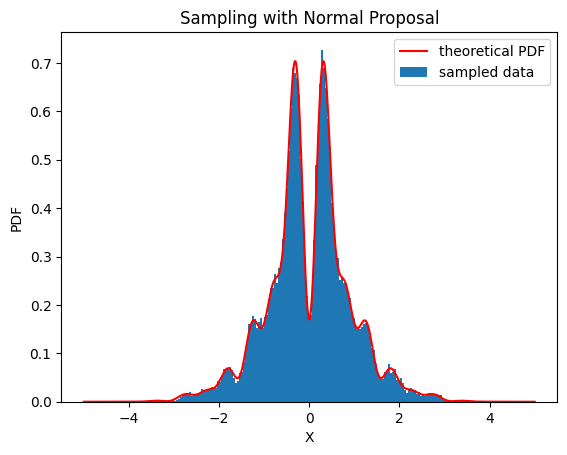
\includegraphics[width=0.55\textwidth]{./figure/p5/new_func.png}
    \caption{Sample $\N(0,1)$ with Acceptance-Rejection method}
\end{figure}

\end{homeworkProblem}

\newpage